\chapter{Approach}\label{chap:approach}
This section is a point by point depiction of the actualized framework utilized in this thesis, which is to detect the Tweets related to Human Migration and its Sentiment. To start with, the undertaking of Mining Twitter data is defined, and the framework is depicted in the sequential order of its working.

\section{Problem Formulation}

Predicting the topic of the Tweet is very challenging work. People discuss or communicate all type of topics from "trending science research" to "current politics" and from "sports events" to "natural calamities" using Twitter. The topics are generic and identifying a specific topic which we need is hard to find from the tweets. The  
Principle point of this approach is a technique to identify the tweets regarding the topic ``human migration". This technique is used to collect the tweets and build a classification model which classifies the new tweets into migration class or otherwise. And the sentiment of these tweets is detected using a sentiment detection model. The solution to the problem can be broken down into stages: Twitter data mining, feature engineering, training, and evaluation stages.


\begin{itemize}
  \item  The first stage, Data is mined from the Twitter. Data mining is a process of extracting information (with intelligent methods) from a data set and transform the information into a comprehensible structure for further use. Here, in this research, information related to human migration from the Twitter dataset is extracted. However, identifying the "human migration" topic in the tweet is difficult, because ground truth value is unknown, collected tweets data cannot be mapped and searched with any population registers. The term "ground truthing" refers to the process of gathering the proper objective data for the test. So, for this reason, data are mined with respect to particular reason namely war, education or work etc. The factors which affect people for migration mentioned in the link.  \footnote{\url{http://www.bbc.co.uk/schools/gcsebitesize/geography/migration/migration_trends_rev2.shtml}  }. The four main important factors which affect human migration are:


\begin{enumerate}
    \item Economic
  \item Social
    \item Political
  \item Environmental
\end{enumerate}
Collecting an unbiased data for all the factors is very difficult. So, only political migration factor is considered in this experiment. The reason only this factor is considered because,  For instance, people can migrate for short period of time for education or work, in this scenario collecting the data from the "LinkedIn" would be more feasible as people would store and share their education and work qualification information. However, Twitter is used by many people who communicate about a political issue and a sufficient amount of data can be collected if Twitter is used.
  
  \item In the Second stage, Meaningful features are extracted from Twitter's JSON data. There are many metadata in Tweet, such as tweet text, created date, user description, and hashtags, among them text of the tweet along with the "user description" is used as a feature and additional features which are calculated using the text of the tweet like migration index, migration percentage are added to feature set. Calculation of the migration index and migration percentage is mentioned in the subsection below.
  
   \item The Tweets are manually annotated as migration tweets (with labels "yes" or "no"), which is used a target labels. The supervised classifier is then trained
using these feature and their corresponding labels in the training stage. Output of this model is fed to another sentiment detection model, which is trained with annotated data \cite{stanford_data}("positive" and "negative" labels) \footnote{\url{http://help.sentiment140.com/for-students/}}
  
  \item In the Fourth stage, These models are evaluated by calculating the Accuracy and the F1 score. The detailed version of evaluation is mentioned in the Evaluation section below.
\end{itemize}



\section{Method}
This section describes the method used in this research. The overview of the research is shown in figure \ref{fig:flowchart_thesis}. The flowchart in the figure \ref{fig:flowchart_thesis} describes us that the approach is divided into two parts. First part(left box of the figure \ref{fig:flowchart_thesis}) classifies the tweets as migration tweets. The second part(right box of the figure \ref{fig:flowchart_thesis}) is detecting the sentiment of tweets. Both the parts use the Twitter data. The output of the first model which are migration tweets is passed to the second model to understand its sentiment which is shown by the arrow from the left box to right box. Details of each step are mentioned in following subsections.

\begin{figure}
    \centering
    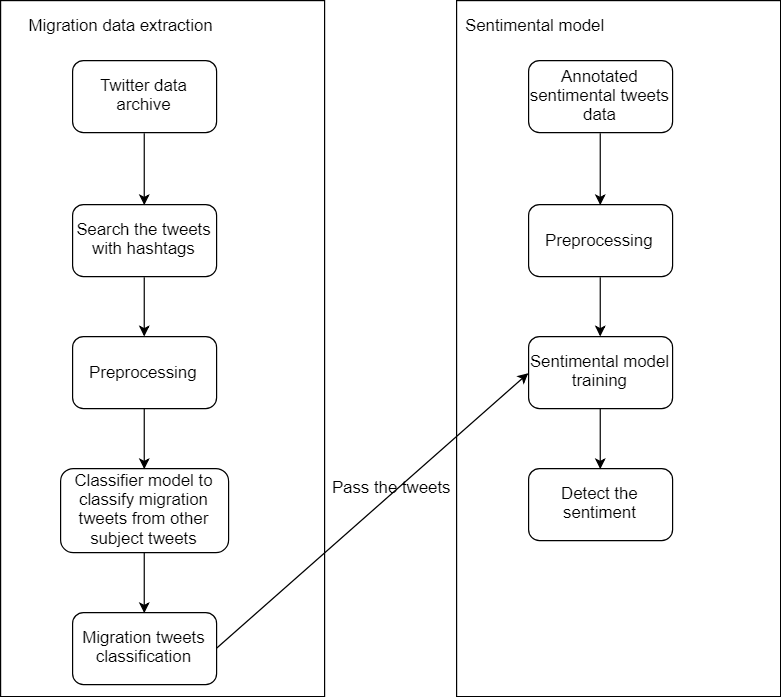
\includegraphics[width=0.75\linewidth]{images/flowchart.png}
    \caption{Flowchart of the approach}
    \label{fig:flowchart_thesis}
\end{figure}
\subsection{Data Collection}
The Twitter company offers various methods for accessing its data. They provide API's(Application Programming Interface) to access data which are of two types such as Rest API's and Streaming API's. Their applications and limitations are mentioned in section (2.1.1). The REST API offers a simple interface and is easy to use for the Twitter functionality. These API's can be used to search for already published tweets, historical tweets. Twitter's streaming API's can be used to search for the tweets which are published in current time. This API's are usually used in an innovative way to collect a huge number of tweet data. For instance, the streaming API can be used to collect the data of any live events and this data can be used to study statistics of people attending or not attending. However, the problem with these two types of API's is, it does not give full access to collect all the public tweets, they offer limitations in accessing the data \footnote{\url{https://developer.twitter.com/en/docs/basics/rate-limiting}}. For full access of the public tweets, commercial packages need to be purchased. The limitations and for the lack of full access of the data, helped me to decide to use the Twitter data archive which is provided in links \footnote{\url{https://archive.org/}} \footnote{\url{https://archive.org/details/twitterstream?and[]=year\%3A\%222016\%22}} \cite{Twitterarchive}. 

The archive.org is a non-profit company, it is trying to build a digital library of internet sites and cultural artifacts in digital form. The data from this website is free to access and is available for researchers, historians, scholars, and the general public. The advantage of using data from this website is, the data can be searched and filtered according to time. for example in this research, November and December months archives from the year 2016 is considered to mine data. 

Once the data archive is chosen, next step searching for the relevant data. But, what is relevant data? for an instance, if the model built, is for ``spam email detection", it cannot be built using the data which is used for detecting ``cancellation of flights". November(2016) and the December(2016) months archives were used. This was used because the hashtags which are used were trending. Another reason why only these two months archives used was, the same hashtags were also applied to search for tweets from other months archives, it did not result in a sufficient number of tweets. Now, other questions arise is how were the hashtags chosen?. Before we choose hashtags, an important point to understand is why people migrate. This is discussed in chapter 3.1 in problem formulation section and only the ``Political" factors are considered in this research and in these factors, war and/or elections are the primary influences for people migrating to different countries. Based on this assumption(political factor), a significant amount of research is done studying these specific topics from news media like online news website and Twitter's trending API's and based on these studies the trending hashtags related to the topics were chosen. Hashtags chosen were ’\#refugee’, ’\#wall’, ’\#Syria’, ’\#syrianrefugee’, ’\#mexicanwall’, ’\#trumpwall’, ’\#immigrants’ and were used as the query parameter to search for tweets. 

The data in the archive is available as a JSON structure. The JSON structure of the tweet is described in the section above \underline{mention the above section}. The archive contains all the tweets which are published in selected time. When the structure of the archive is analyzed, Every line in the file was a tweet object which is in JSON format. Twitter's JSON data contains many metadata one such is `entities' metadata. This metadata contains arrays of common things in Tweets such as hashtags, user mentions, links, stock tickers (symbols), Twitter polls, and attached media. Structure of the entities metadata is shown in the figure \ref{fig:entities}. The hashtags metadata contains all the hashtags which are used in tweet's text. This structure can be used to search for the hashtags in the tweet. This idea is applied to filter tweets matching the list of hashtags which were chosen. So, a script was designed which take each line of the JSON file as the input and search the ``entity" metadata for the presence of the pre-collected hashtags list. If a match is obtained, the tweet object is stored in a CSV file. One more query parameter which is used for searching filter is the language of the tweet, only ``English" language tweet were searched. This was performed by checking the ``Lang" metadata in the tweet JSON object. The Flowchart of the tweets filter is shown in the figure \ref{fig:tweetsfilter}.


\begin{figure}
    \centering
    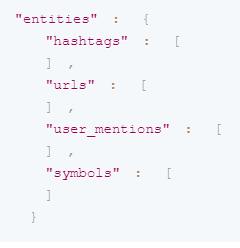
\includegraphics[width=0.5\linewidth]{images/entities.png}
    \caption{Entities metadata in tweet's JSON}
    \label{fig:entities}
\end{figure}

\begin{figure}
    \centering
    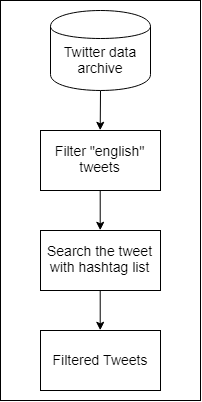
\includegraphics[width=5cm\linewidth,height=7cm]{images/filtertweets.png}
    \caption{Flowchart of the tweets filter.}
    \label{fig:tweetsfilter}
\end{figure}


\paragraph{Datasets}
The dataset has been acquired through the filtering process shown in the figure \ref{fig:tweetsfilter}. The dataset contains 1276 tweets collected using the hashtag list (’\#refugee’, ’\#wall’, ’\#Syria’, ’\#syrianrefugee’, ’\#mexicanwall’, ’\#trumpwall’, ’\#immigrants’). Hereinafter this dataset is referred to as the migration data-set. Each tweet is pre-classified manually as migration ``yes" and migration ``no" classes, in addition, the sentiment of these tweets is also annotated with ``positive" and ``negative" classes. Only two classes are selected because the binary classifier model is built using this. Text classification techniques usually have a third class ``irrelevant" or ``neutral" class. In my research, however, the third class is not considered for the reasons, a number of tweets in the data set are smaller and if the third classes is chosen some data is lost. Moreover, while annotating if the tweets belong to the ``irrelevant" or ``neutral" class, they are classified to ``negative" class. The classes of the tweets in this data-set are annotated by my colleagues who understand and speaks English fluently. The data-set was shared with five of my colleagues and the average of the annotation was considered as the final class. The distribution of the two classes `yes' and `no' classes is shown in figure \ref{tab:DistMigrationClass}. The distribution of the two classes `positive' and `negative' classes is shown in figure \ref{tab:Distribution of sentiment class}.



\begin{table}[]
\centering
\begin{tabular}{lllll}
\cline{1-2}
\multicolumn{1}{|l|}{Classes}   & \multicolumn{1}{l|}{number of tweets} &  &  &  \\ \cline{1-2}
\multicolumn{1}{|l|}{``yes"} & \multicolumn{1}{l|}{449}  &  &  &  \\ \cline{1-2}
\multicolumn{1}{|l|}{``no"}   & \multicolumn{1}{l|}{826}  &  &  &  \\ \cline{1-2}
                            &                           &  &  & 

\end{tabular}
\caption{Distribution of migration class}
\label{tab:DistMigrationClass}
\end{table}

\begin{table}[]
\centering
\begin{tabular}{lllll}
\cline{1-2}
\multicolumn{1}{|l|}{Classes}   & \multicolumn{1}{l|}{number of tweets} &  &  &  \\ \cline{1-2}
\multicolumn{1}{|l|}{``positive"} & \multicolumn{1}{l|}{565}  &  &  &  \\ \cline{1-2}
\multicolumn{1}{|l|}{``negative"}   & \multicolumn{1}{l|}{710}  &  &  &  \\ \cline{1-2}
                            &                           &  &  & 
\label{tab:Distribution of sentiment class}
\end{tabular}
\caption{Distribution of sentiment class}
\label{tab:DistsentimentClass}
\end{table}

Besides the migration data-set, two additional data-set is collected. First, for sentiment detection model and second, for evaluation of the classification model for migration. For the Sentiment detection model, annotated sentiment data from \cite{stanford_data} is used. This data-set contains 1.6 million tweets, of which it contains  800000 tweets of each class. This data is cleaned and sentiment classification model is built. Another data-set is collected is from \cite{CanadianmMigrationDataset}. This is a data-set for Canadian migration collected on Twitter. This data-set contains 800 tweets which are classified into migration tweets, for which additional 800 random tweets are added to balance the data set. The 800 additional tweets are classified as non-migration tweets. For this data-set, the migration data-set is added and the accuracy of the model built with combined data-set is compared with the accuracy of the model built with migration data-set. 



\subsection{Prepossessing} \label{preprocessing}
The overall system output standards depend on the quality of the input data. The additional information provided by Twitter data(example: user mentions, URLs) does not provide many useful properties. Hence to enhance the quality of the input information a pre-preparing stage is required. The prepossessing step applies to all three collected data sets. Since the data sets only contain Twitter data, the prepossessing step is common for all data sets. The prepossessing process involves many steps: language check, removal of duplicate, merging tweet message and user description, message cleaning which is shown in the figure \ref{fig:preprocessing}. 

The tweets in the data-set are present in JSON format, so each line of the file is a JSON object. The prepossessing script reads the file line by line, parses each line into a JSON object and acts as follows.

\subsubsection{Language check}
Since Twitter is used worldwide, the messages are generally available in almost any language. Text analysis and classification makes use of linguistic content and language, therefore, language plays a key role. The Language importance in any text classification is discussed in section \ref{chap:background}. In this research, I restrict my scope to tweets in English only. Non-English tweet messages are therefore discarded before any experimental steps performed on the data-set. 
Language detection is one of the interesting and challenging fields in Natural language processing(NLP). Researches use translators to convert the message to a single language for text analysis, usually to English.
\begin{figure}
    \centering
    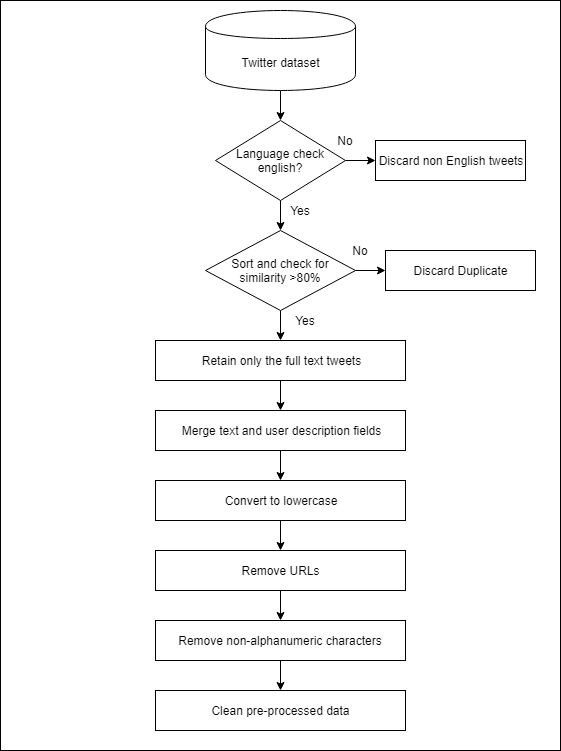
\includegraphics[width=10cm\linewidth,height=13cm]{thesis_template/images/preprocessing.png}
    \caption{Prepossessing steps}
    \label{fig:preprocessing}
\end{figure}
However, to implement language check and to filter only English language tweet messages. I take advantage of the Twitter data structure. Twitter stores each message as a JSON object and it contains ``Lang" metadata which informs that, to which language the message belongs to. A script is implemented to check this before the tweets are passed on to the next prepossessing stage. This script checks the ``Lang" metadata for the keyword ``en" which signifies the language is English and discards other keywords(Example, ``es" for Spanish, ``jp" for Japanese). By the end of this script, only English tweets are collected passed on to duplicate message checking step.  

\subsubsection{Removal of duplicate messages}
After the Language filter, the next step which is used in research is the duplicate check of the tweet messages. There is a lot of research on the use of duplicates in the data set in the field of data science. There is no hard rule to remove the duplicates in the data-set. Sometimes the machine learning model improves the accuracy, and at times the model is over-fitted. Since, word frequency is used in this research, allowing the duplicate message simply increases the word count and the classifier model
achieves a very low training error by learning to be very good at same data that repeats a lot in the training set.

Another important reason why duplicates need to be removed especially in this research is the Twitter's functionality of ``re-tweeting". A retweet is just a repost of the tweet of another Twitter user on your own profile. Like hash-tags, retweets are a community-driven phenomenon on Twitter that helps to improve the service and make it easier for people to talk. So after searching the tweets with hash-tags and filtering only English tweet, duplicate messages tweet is implemented.

This duplicate checker is implemented using a simple idea to sort the text of tweets first and to compare two consecutive texts for similarity. The two consecutive texts shall only be considered similar if they are 80\% similar. If the two tweets are similar first tweet is saved and the second tweet is discarded. Flowchart of the process is shown in figure \ref{fig:duplicatechk}. Sorting and similarity check is implemented using the `pandas' python library\footnote{\url{https://pandas.pydata.org/pandas-docs/version/0.17.0/generated/pandas.DataFrame.sort_values.html}} and `difflib' python library \footnote{\url{https://docs.python.org/2/library/difflib.html}}.

\begin{figure}
    \centering
    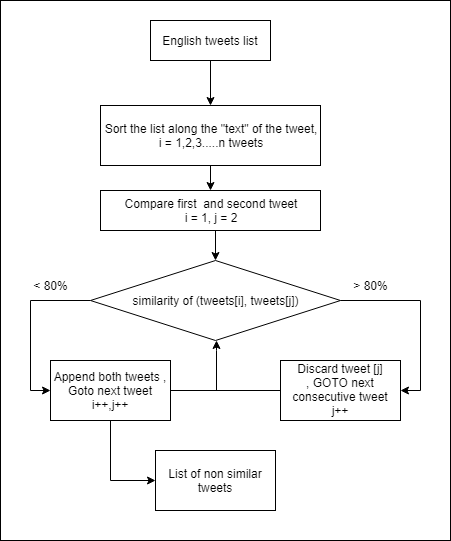
\includegraphics[width=10cm\linewidth,height=10cm]{thesis_template/images/duplicatecheck.png}
    \caption{Removal of duplicate messages}
    \label{fig:duplicatechk}
\end{figure}

\subsubsection{Merge text and Description fields}

One element which made Twitter popular social media network is that it limits your posts to 140 characters(recently characters length is increased to 280). However, this could be disadvantageous for data scientists who try to extract information from the tweet message. Since only 140 characters and people try to shorten the message using acronyms and a lot of unwanted information is also present in a tweet which includes URL and users mention. This research, therefore, combines the text of the tweet message with a user description, which increases the number of characters. User description is another metadata which is present in Twitter JSON structure. In addition, I could just get some more information about user migration by including his/her description. This implement is a simple task, a script just checks whether the user description field has a value if present it is merged with the message.

\subsubsection{Message cleaning}
In this step, the text in the tweet message is cleaned. The message of the Tweet contains only 140 characters, To this user description, is added. But, as mentioned before, These limited size constraints make people shorten the message using acronyms and wrong spelling. 
In order to create a purer data set for the classifier training, message cleaning techniques are used. First, all the characters are converted to lowercase. Once it is normalized into single basic structure, several techniques are applied such as remove URL's, remove non-alphanumeric characters. This is implemented using the regular expression, which is an efficient string replacement algorithm. Another action was performed was the removal of the stop words. Stop words are the commonly occurring words(such as "a", "the", "is", "in") because it just adds the number of words and provide less information. also takes processing time. This was done using the NLTK library which is available in python language, it has the stopwords list of for 16 different languages. 
\subsubsection{Manual Annotations}
The Data-sets collected are shared with three of my colleagues to annotate. Each annotator annotates the tweet with 2 labels. One as migration "yes" or "no" and second for the sentiment of the tweets "pos" or "neg". I take a mean of those annotations and assign the labels for each collected tweet.

\subsection{Feature engineering} \label{featureengineering}


 
Before classifying tweets using the machine learning approach, features must be extracted after the prepossessing step. Without the right set of features, even the powerful machine learning algorithm results badly. This was understood from the literature survey. As mentioned in the problem formulation section, I am building two separate models, and both the models follow the same feature extraction methods, but for the migration tweets, the classifier model has two additional features.

In my research, I have created a heterogeneous feature set. Heterogeneous feature set advantages are discussed in \ref{chap:background}. Feature set contains, features extracted from the text using the count vector technique, and additional two feature are added to this feature, that is ``Migration index" and ``Migration percentage".   

I decided to create a feature vector using count vectorizer. This technique is simple to implement and decision to use this was based on the performance. The count vector is implemented using the "CountVectorizer" library from scikit learn \cite{scikit-learn}. The CountVectorizer library offers a simple way to tokenize a collection of text documents and build a vocabulary of known words, but also to encode new documents using that vocabulary. This library takes text document as input and to learn about the document a fit function is executed. Then an encoded vector with an entire vocabulary length and an integer count for the number of times each word appeared in the document is returned. The returned vector is a sparse as it contains many zeroes. This sparse matrix is handled using the sparse library from scipy.org.

Migration index" is computed based on the Dictionary. This dictionary is a list of words which are related to migration along with corresponding weights which are manually assigned based on the severity level which is 1 to 5, 1 being negligible and 5 being extremely related to migration. This severity is calculated based on the word frequency. A word-cloud is generated with the collected tweets "text" and the severity number is assigned to the words based on the most frequently occurring word.
 I check all the tweets for the presence of words from this dictionary if present it gets the corresponding weights of all those words and mean is calculated for those weights. This mean value is "Migration index". 
 


Presence of Migration term in tweet message alone cannot necessarily mean the text is related
to Human migration. The text/tweet can be considered more related to migration if the migration word is directed at a particular individual, a group of
people, race, country, religion etc. For this reason, I also created a list of pronouns and collective nouns, with this ”Migration percentage” is calculated based on the presence of Migration word along with pronouns or collective nouns.




Finally, the Count vector feature, migration index, migration percentage are combined and used a feature set, which is shown in the fig \ref{fig:featureeng}. This set and its corresponding classes are split in test and training set and used as an input to the supervised machine learning algorithm, which is discussed in the next section.

\begin{figure}
    \centering
    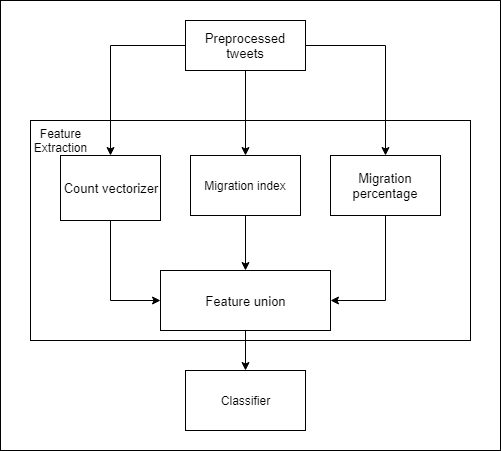
\includegraphics[width=10cm\linewidth,height=10cm]{thesis_template/images/featureengineering.png}
    \caption{Migration model feature engineering}
    \label{fig:featureeng}
\end{figure}
    

Location is obtained using the "Geopy" python library. The user location is passed to "Geopy" library to get latitude and longitude. 



\subsection{Data-set split}
Before we can train any model, we think about how to split the data first. There are two types of splitting the data such as:
\begin{enumerate}
    \item Test/Train sets
  \item Test/Train/Dev sets
\end{enumerate}
The definitions of the three terms are as following:
\begin{itemize}
     \item Train set: Sample of data used of learning.
 
    \item Test set: Sample of data used for calculating the accuracy of the model.
      \item Dev set: Sample of data which is used for unbiased evaluation of the model performance.
\end{itemize}

From now on I will be discussing the two models, firstly migration detection and second, sentiment detection. For the migration detection model, I decided to divide the data set in test and train sets for the migration detection model, Because there were fewer tweets. It was split as 75\% train and 25\%test sets. The data is divided into the test, train and dev sets for the sentiment detection model because more tweets are available and this was split as 98\% train set, 1\%test set, and 1\% dev set.
Distribution of the Tweets after the train/test split for migration data-set is shown in the table \ref{tab:Distmigrationdataset}. Distribution of the Tweets after the train/test/dev split for sentiment data-set is shown in the table \ref{tab:Distsentimentdatset}. This split was implemented using the ``model selection" library from the scikit learn \cite{scikit-learn}.


\begin{table}[]
\centering
\begin{tabular}{lllll}
\cline{1-2}
\multicolumn{1}{|l|}{Sets}   & \multicolumn{1}{l|}{number of tweets} &  &  &  \\ \cline{1-2}
\multicolumn{1}{|l|}{Train} & \multicolumn{1}{l|}{956}  &  &  &  \\ \cline{1-2}
\multicolumn{1}{|l|}{Test} & \multicolumn{1}{l|}{319}  &  &  &  \\ \cline{1-2}
\multicolumn{1}{|l|}{Total}   & \multicolumn{1}{l|}{1275}  &  &  &  \\ \cline{1-2}
                            &                           &  &  & 
\label{tab:Distribution of sentiment class}
\end{tabular}
\caption{Distribution of train/test split for migration data-set}
\label{tab:Distmigrationdataset}
\end{table}

\begin{table}[]
\centering
\begin{tabular}{lllll}
\cline{1-2}
\multicolumn{1}{|l|}{Sets}   & \multicolumn{1}{l|}{number of tweets} &  &  &  \\ \cline{1-2}
\multicolumn{1}{|l|}{Train} & \multicolumn{1}{l|}{1568000}  &  &  &  \\ \cline{1-2}
\multicolumn{1}{|l|}{Dev} & \multicolumn{1}{l|}{16000 }  &  &  &  \\ \cline{1-2}
\multicolumn{1}{|l|}{Test} & \multicolumn{1}{l|}{16000 }  &  &  &  \\ \cline{1-2}
\multicolumn{1}{|l|}{Total}   & \multicolumn{1}{l|}{1600000}  &  &  &  \\ \cline{1-2}
                            &                           &  &  & 
\label{tab:Distribution of sentiment class}
\end{tabular}
\caption{Distribution of train/dev/test split for migration data-set}
\label{tab:Distsentimentdatset}
\end{table}


\subsection{Classification}
As mentioned above, this project incorporates two classifier models. One, migration detection classifier, another model for sentiment detection. The tweets classified as migration tweets are transferred to the second model in order to detect their sentiment. The feature extraction method is slightly different for both models. For the migration model, the feature set contains a tweet message count vector, migration index, and migration percentage. However, the sentiment detection model contains only the tweet message count vector as a feature set. So, these feature set are passed as the input to the classifier. To classify tweets, there are many algorithms. However, I have compared the accuracy of three classifier algorithms, such as naive Bayes, logistic regression and decision trees. The classifier learns a pattern based on the inputs and classifies new samples into specific classes.



\subsection{Evaluation} \label{eval}
Once the problem is set and the data is prepared, the machine learning model is applied to solve the problem. Before applying the machine learning model a test harness needs to be defined. The test harness is the data which is used to test the trained algorithm. The performance of the algorithm is measured using the test harness, performance metrics are discussed in Section \ref{scoringmetrics}.

Two types of evaluation are conducted in this research,
\begin{enumerate}
    \item To evaluate the migration detection model. This is conducted by 2 methods:
    \begin{itemize}
        \item First method : 
        The classifier is evaluated using the test data set, by calculating the performance metric.
        \item Second method :
         This method is undertaken to check the performance of the algorithm based on the data set, but for the same problem of detecting the migration tweets.
        \begin{itemize}
       
            \item With Canadian migration data \footnote{\url{https://data.world/wendyhe/tweets-on-canada-immigration}}, which is a migration-related data-set where each tweet in the data-set belongs to migration (label "yes"). This data-set contains 800 tweets. Along with this another 800 tweets which belong to random categories are added, where these tweets are manually picked which are not related to migration (label "no"). 
            \item With these 1600 random and Canadian tweets, migration data set which are collected in the data collection step are combined together totaling to around 2600 tweets.
            \item A binary classifier will be trained from the above tweets, and the accuracy of this model and the model which is built only from migration data-set is compared.
        \end{itemize}
        
    \end{itemize}


    \item Evaluating the Sentiment analysis is performed with the "test data set",
by calculating the F1 score, Accuracy.
\end{enumerate}